\section{夹逼准则}
\begin{theorem}
%@see: 《数学分析(上册)》(陈纪修) P76 定理3.1.3
%@see: 《高等数学(第六版 上册)》 P50 准则I'
设函数\(f,g,h\)满足\begin{itemize}
	\item \((\exists\rho>0)
	[0<\abs{x-x_0}<\rho \implies g(x) \leq f(x) \leq h(x)]\),
	\item \(\lim_{x \to x_0} g(x) = \lim_{x \to x_0} h(x) = A\),
\end{itemize}
则\(\lim_{x \to x_0} f(x) = A\).
\begin{proof}
对于\(\forall\epsilon>0\),
有\begin{gather*}
	\lim_{x \to x_0} h(x) = A
	\implies
	(\exists\delta_1>0)
	(\forall x\in\mathbb{R})
	\left[
		\begin{array}{rl}
			0<\abs{x-x_0}<\delta_1
			&\implies
			\abs{h(x)-A}<\epsilon \\
			&\implies
			h(x)<A+\epsilon
		\end{array}
	\right], \\
	\lim_{x \to x_0} g(x) = A
	\implies
	(\exists\delta_2>0)
	(\forall x\in\mathbb{R})
	\left[
		\begin{array}{rl}
			0<\abs{x-x_0}<\delta_2
			&\implies
			\abs{h(x)-A}<\epsilon \\
			&\implies
			A-\epsilon<g(x)
		\end{array}
	\right].
\end{gather*}
取\(\delta=\min\{\delta_1,\delta_2,\rho\}\),
则\[
	(\forall x\in\mathbb{R})
	[
		0<\abs{x-x_0}<\delta
		\implies
		A-\epsilon < g(x) \leq f(x) \leq h(x) < A+\epsilon
	],
\]
即\(\lim_{x \to x_0} f(x) = A\).
\end{proof}
\end{theorem}

\begin{example}[重要极限I]
试证:\begin{equation}\label{equation:极限.重要极限I}
\lim_{x\to0} \frac{\sin x}{x} = 1.
\end{equation}
\begin{proof}
如图所示,
\begin{center}
	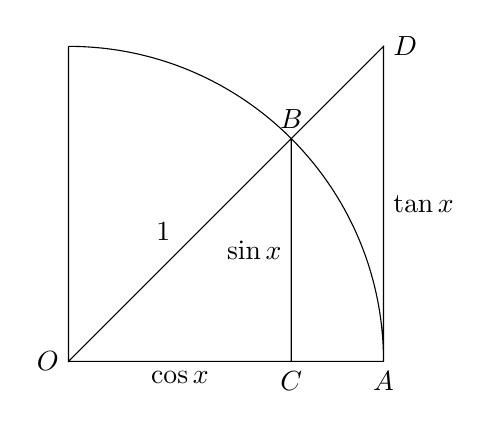
\begin{tikzpicture}
		\pgfmathsetmacro{\r}{4}
		\pgfmathsetmacro{\cx}{\r/sqrt(2)}
		\coordinate(O)at(0,0);
		\coordinate(A)at(\r,0);
		\coordinate(B)at(\cx,\cx);
		\coordinate(C)at(\cx,0);
		\coordinate(D)at(\r,\r);
		\draw (O)node[left]{\(O\)}
			--(C)node[below]{\(C\)}node[midway,below]{\(\cos x\)}
			--(A)node[below]{\(A\)}arc[start angle=0,end angle=90,radius=\r] (C)
			--(B)node[above]{\(B\)}node[midway,left]{\(\sin x\)}
			--(O)node[midway,above left]{\(1\)}
			--(0,\r)
			(B)
			--(D)node[right]{\(D\)}
			--(A)node[midway,right]{\(\tan x\)};
	\end{tikzpicture}
\end{center}
由于在\(0 < x < \pi/2\)时,\[
	0 < \sin x < x < \tan x
	\implies
	1 < \frac{x}{\sin x} < \frac{1}{\cos x}
	\implies
	\cos x < \frac{\sin x}{x} < 1.
\]
因为\(\lim_{x\to0}\cos x = 1\),
所以由\hyperref[theorem:极限.夹逼准则]{夹逼准则}可知,
\(\lim_{x\to0} \frac{\sin x}{x} = 1\).
\end{proof}
\end{example}

%TODO: 函数\(\frac{\sin x}{x}\)的图像
% \begin{figure}[ht]
% 	\centering
% 	\begin{tikzpicture}
% 		\begin{axis}[
% 			xmin=-4*pi,xmax=4*pi,
% 			ymin=-.5,ymax=1.2,
% 			width=\textwidth,
% 			height=.3\textheight,
% 			grid=both,
% 			xlabel=$x$,
% 			ylabel=$y$,
% 			enlargelimits,
% 			axis lines=middle,
% 			xtick={3.14,6.28,9.42,-3.14,-6.28,-9.42},
% 			xticklabels={$\pi$,$2\pi$,$3\pi$,$-\pi$,$-2\pi$,$-3\pi$},
% 		]
% 			\begin{scope}[samples=50,thick,red]
% 				\addplot[domain=.01:4*pi]{sin(deg(x))/x};
% 				\addplot[domain=-4*pi:-.01]{sin(deg(x))/x};
% 			\end{scope}
% 			\filldraw[draw=black,fill=white](0,1)circle(1pt);
% 		\end{axis}
% 	\end{tikzpicture}
% 	\caption{函数\(y=\frac{\sin x}{x}\)的图像}
% 	\label{figure:极限.函数[y=sin(x)/x]的图像}
% \end{figure}

% \begin{example}
% 求:\(\lim_{x\to0} \frac{\tan x}{x}\).
% \begin{solution}
% \(\lim_{x\to0} \frac{\tan x}{x}
% = \lim_{x\to0} \left(\frac{\sin x}{x} \cdot \frac{1}{\cos x}\right)
% = \lim_{x\to0} \frac{\sin x}{x} \cdot \lim_{x\to0}\frac{1}{\cos x}
% = 1\).
% \end{solution}
% \end{example}

% \begin{example}
% 求:\(\lim_{x\to0} \frac{1 - \cos x}{x^2}\).
% \begin{solution}
% \(\lim_{x\to0} \frac{1 - \cos x}{x^2}
% = \lim_{x\to0} \frac{2 \sin^2\frac{x}{2}}{x^2}
% = \frac{1}{2} \lim_{x\to0} \frac{\sin^2\frac{x}{2}}{\left(\frac{x}{2}\right)^2}
% = \frac{1}{2} \left(\lim_{x\to0} \frac{\sin \frac{x}{2}}{\frac{x}{2}}\right)^2
% = \frac{1}{2}\).
% \end{solution}
% \end{example}

% \begin{example}
% 求:\(\lim_{x\to0} \frac{\arcsin x}{x}\).
% \begin{solution}
% 令\(t = \arcsin x\),
% 则\(x = \sin t\).
% 当\(x\to0\)时,
% 有\(t\to0\).
% 于是由复合函数的极限运算法则得\[
% 	\lim_{x\to0}\frac{\arcsin x}{x}
% 	= \lim_{t\to0}\frac{t}{\sin t}
% 	= 1.
% \]
% \end{solution}
% \end{example}
